\section{Exploratory Data Analysis}

% As part of the EDA, we checked the class distribution, the distribution of features amongst the different classes and analysed the first two principle components of the data. 

% As part of our exploratory data analysis (EDA), we first examined scaled features and how well they each divide glass fragments based on their class. Second, we looked at a scatter plot of the first two principal components, which explain $51 \%$ of variance to examine the same thing as in the first example. Our overall goal was to use this analysis for our decisions during modelling part of the project.
\subsection{Class Distribution}
Figure \ref{class_distribution} shows the class distribution in the training and test split. The distribution of classes were roughly the same amongst the two splits. This was important to notice, since evaluating a classifier that was trained on data with a class distribution highly different from the testing set, would result in an inaccurate estimations for the out-of-sample performance.
Apart from that, a strong imbalance in the six observed classes became obvious. While the two majority classes 1 and 2 made up more than 65\% of the entire data, the underrepresented classes 3, 5 and 6 all combined accounted for less than 25\% of all data points. This imbalance might pose challenges when it comes to building a classifier correctly classifying the minority classes. 
\newline

\begin{figure}[ht]
\centering
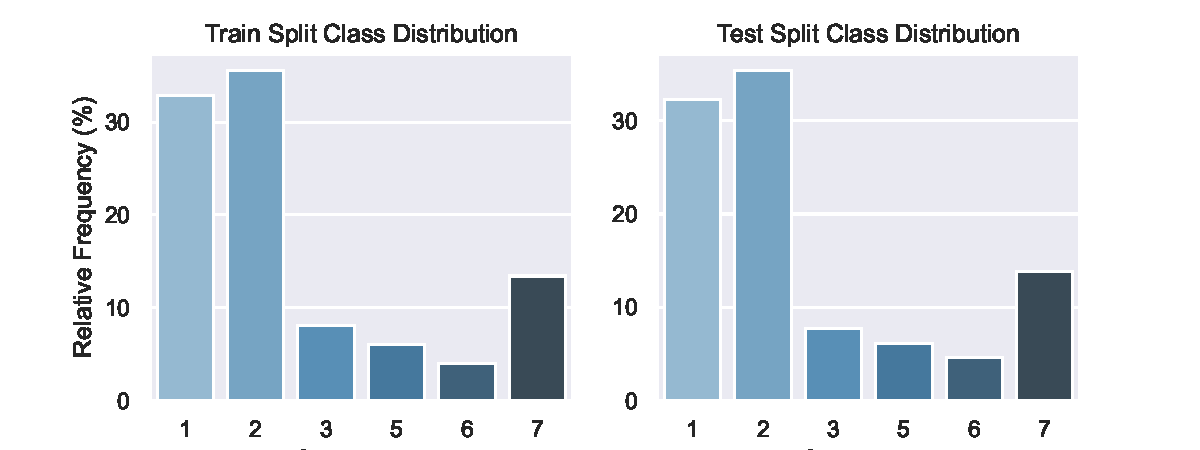
\includegraphics[scale=0.6]{figures/class_distribution.pdf}
\caption{Class Distribution in (a) Training Split and (b) Test Split}
\captionsetup{justification=centering,margin=2cm}
\label{class_distribution}
\end{figure}

\begin{comment}
\subsection{Feature Distribution}
Table \ref{feature_distribution} shows the five-number summary of each feature computed from the training and test split combined. It becomes evident, that all types of glass fragments are primarily composed of the chemical compound \textit{silicone} (between $\sim 69\%$ and $\sim 75\%$) and \textit{sodium} (between $\sim 10\%$ and $\sim 17\%$). Interestingly, the RI, which was expected to have a high variance amongst different types of glass fragments, has a small difference between the maximum and minimum value. Looking at the feature distribution for each class will reveal, how well each feature separates the six classes.
\newline

\begin{table}[!ht]
  \small
  \centering
\begin{tabular}{ c | c c c c c}
 \toprule
 Feature &  Min  & Lower Quartile  &  Median  &.  Upper Quartile  &   Max\\
 \midrule
 RI   &   1.51  &  1.52   & 1.52  & 1.52  & 1.53 \\
 Na   &   10.73 &  12.91  & 13.30 & 13.83 & 17.38 \\
 Mg   &   0.00  &  2.12   & 3.48  & 3.60  & 4.49 \\
 Al   &   0.29  &  1.19   & 1.36  & 1.63  & 3.50 \\
 Si   &   69.81 &  72.28  & 72.79 & 73.09 & 75.41 \\
 K    &   0.00  &  0.12   & 0.56  & 0.61  & 6.21 \\
 Ca   &   5.43  &  8.24   & 8.60  & 9.17  & 16.19 \\
 Ba   &   0.00  &  0.00   & 0.00  & 0.00  & 3.15 \\
 Fe   &   0.00  &  0.00   & 0.00  & 0.10  & 0.51 \\
 \bottomrule
\end{tabular}
\captionsetup{justification=centering,margin=2cm}
\caption{Five-Number-Summaries for all Features}
\label{feature_distribution}
\end{table}
\end{comment}

\subsection{Distribution of Features For Each Class}
Figure \ref{feature_distribution_classes} displays the distribution of each feature in each class, which gives an intuition of how well each feature separates the classes.

\begin{figure}[ht]
\centering
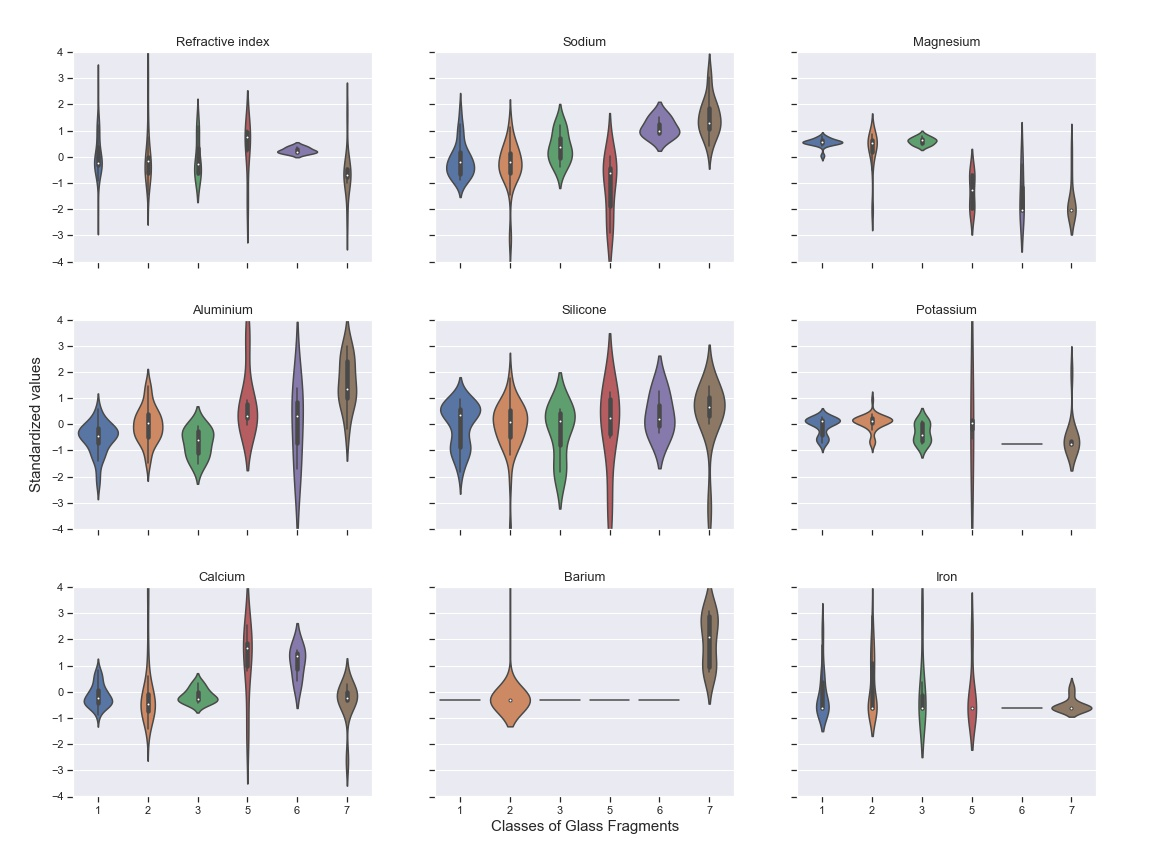
\includegraphics[scale=0.3]{figures/fdist_violin.jpg}
\captionsetup{justification=centering,margin=2cm}
\caption{Standardised Distribution of Features for each Class}
\label{feature_distribution_classes}
\end{figure}

The nine plots show that the different features are differently well-suited for classifying the glass fragments. Features such as \textit{silicone} do not seem to perform well, as there is little variation in the distribution of the feature in the six glass types. On the opposite, features such as \textit{calcium}, \textit{barium}, \textit{magnesium} or the \textit{RI}, seem to be better suited, as they separate subsets of types of glass fragments. However, it can be summarised, that there does not exist a single feature, that can be used to perfectly separate the classes. It is therefore likely that the classifier will need to be trained on a combination of features.


\subsection{Principal Component Analysis}
%Principle component analysis (PCA) is an unsupervised data exploration tool to transform a set of features into a set of representative features - called principle components - that collectively explain most of the variability in the original set. 
Figure \ref{pca} visualises the first two principle components of the data set. The visualisation provides an understanding of the difficulty of the classification problem.

It is evident, that the classification problem is not trivial. The first two principle components reveal, that glass types for similar real-world purposes, ie. class 1, 2 and 3 all being windows, have related feature distributions and are thus overlapping in the first two principle components. This is likely to pose a challenge to the classifier. In contrast,  class $7$ (headlamp) is well-separated and is therefore expected to be easier to classify correctly.

Another challenge might be the under-representation of classes 3, 5 and 6. It will be difficult for the model to learn the patterns in the data for these classes, especially in the case of class 3 being in the middle of the point clouds of the majority classes 1 and 2.

\begin{figure}[ht]
\centering
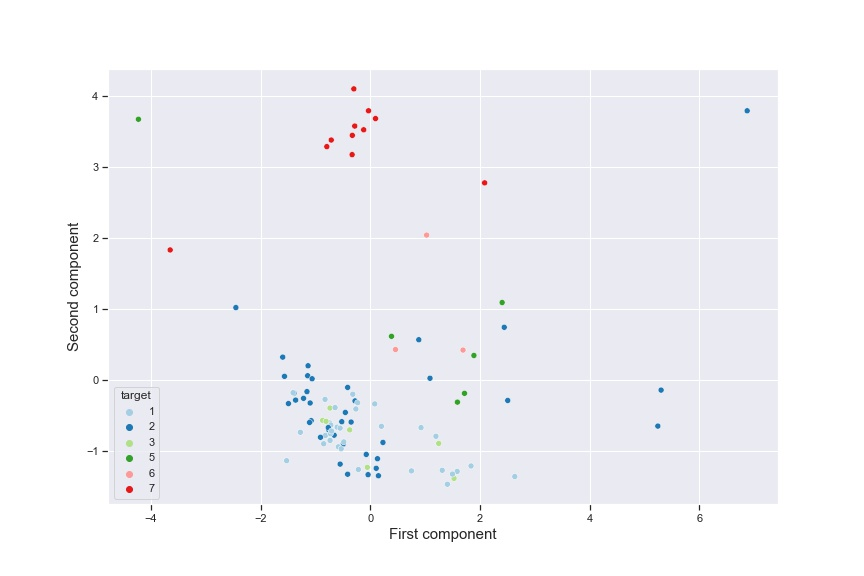
\includegraphics[scale=0.35]{figures/pca_best2_scatter.jpg}
\captionsetup{justification=centering,margin=2cm}
\caption{Scatter Plot of first two Principal Components of Training Split}
\label{pca}
\end{figure}
\newpage